\documentclass{article}

\usepackage{graphicx}
\usepackage{amsfonts,amsmath,amssymb,amsthm}
\usepackage{url}
\usepackage[usenames]{color}
\usepackage[]{algorithm2e}
\usepackage{minted}
\usepackage{booktabs}
\usepackage{amssymb}
\newcommand{\figref}[1]{Figure~\ref{#1}}

\pagestyle{empty} \addtolength{\textwidth}{1.0in}
\addtolength{\textheight}{0.5in} \addtolength{\oddsidemargin}{-0.5in}
\addtolength{\evensidemargin}{-0.5in}
\newcommand{\ruleskip}{\bigskip\hrule\bigskip}
\newcommand{\nodify}[1]{{\sc #1}} \newcommand{\points}[1]{{\textbf{[#1
points]}}}

\newcommand{\bitem}{\begin{list}{$\bullet$}%
{\setlength{\itemsep}{0pt}\setlength{\topsep}{0pt}%
\setlength{\rightmargin}{0pt}}} \newcommand{\eitem}{\end{list}}

%\input{../../defs}

\newcommand{\G}{\mathcal{G}}

%\newcommand{\bE}{\mbox{\boldmath $E$}}
%\newcommand{\be}{\mbox{\boldmath $e$}}
%\newcommand{\bU}{\mbox{\boldmath $U$}}
%\newcommand{\bu}{\mbox{\boldmath $u$}}
%\newcommand{\bQ}{\mbox{\boldmath $Q$}}
%\newcommand{\bq}{\mbox{\boldmath $q$}}
%\newcommand{\bX}{\mbox{\boldmath $X$}}
%\newcommand{\bY}{\mbox{\boldmath $Y$}}
%\newcommand{\bZ}{\mbox{\boldmath $Z$}}
%\newcommand{\bx}{\mbox{\boldmath $x$}}
%\newcommand{\by}{\mbox{\boldmath $y$}}
%\newcommand{\bz}{\mbox{\boldmath $z$}}

\newcommand{\true}{\mbox{true}}
\newcommand{\Parents}{\mbox{Parents}}

\newcommand{\ww}{{\bf w}}
\newcommand{\xx}{{\bf x}}
\newcommand{\yy}{{\bf y}}
\newcommand{\real}{\ensuremath{\mathbb{R}}}


\newcommand{\eat}[1]{}

\newcommand{\CInd}[3]{({#1} \perp {#2} \mid {#3})}
\newcommand{\Ind}[2]{({#1} \perp {#2})}

\setlength{\parindent}{0pt} \setlength{\parskip}{0.5ex}
\begin{document}
\pagestyle{myheadings} \markboth{}{DS-GA-1005/CSCI-GA.2569 Problem Set
  5  Zhuoru Lin's answer }

{\LARGE
\begin{center}Inference and Representation, Fall 2017\end{center}
}

{\Large
Problem Set 5: Hamiltonian Monte-Carlo
}
\begin{center}
Zhuoru Lin\\
zlin@nyu.edu
\end{center}


%{\bf Selected solutions}\\
\ruleskip 
{\em Disclaimer: 
I adhered to NYU honor code in this assignment. }
\begin{enumerate}
\item 
To show $\mathcal{L}(\textbf{v}, \textbf{x})$ is convex given $\textbf{v}$, we show the second derivative of $\mathcal{L}$ with respect to $\textbf{v}$ is larger than zero for all $\textbf{v}$. In fact:

\begin{equation}
\frac{\partial^2\mathcal{L}}{\partial\mathbf{v}^2} = M.
\end{equation}
By definition $M$ is a positive matrix. Therefore $\mathcal{L}$ is convex with respect to $\textbf{v}$.
\pagebreak
\item 
We use the fact that the pointwise suprenum of a set of convex functions is also convex. Consider any $y \in \Omega$, we must have $<y, p>+ f(y)$ is convex with respect to $p$, therefore the convex conjugate:
\begin{equation}
f^{*}(p) = \sup_{y}(<y, p>+f(x))
\end{equation}
\pagebreak
is convex.
\item 
By the definition of $\mathcal{L}$ and $\textbf{p}$ we have:
\begin{equation}\label{def_p}
\textbf{p} = \frac{\partial \mathcal{L}}{\partial \textbf{v}} = M \textbf{v}.
\end{equation}
The convex conjugate of $\mathcal{L}(\textbf{v})$ is:
\begin{align*}
\mathcal{L}^{*} (v) &= \sup_{v} [<v, p> - \mathcal{L}(\mathbf{v})]\\
&= \sup_{v}[<v, Mv> - \frac{1}{2} <v, mv> + U(\textbf{x})]\\
&= \sup_{v} [ \frac{1}{2} <v, mv> + U(\textbf{x}) ]
\end{align*}
There fore the Hamilton $\mathcal{H}$ must have the form:
\begin{equation}\label{def_H}
\mathcal{H}(\textbf{p}, \textbf{x}) = \frac{1}{2} <\textbf{p}, M^{-1} \textbf{p}> + U(\textbf{x})
\end{equation}
\pagebreak

\item 
By the definition of $\mathcal{H}$ (equation \ref{def_H}), we have:

\begin{equation}\label{def_hamilton_eq_1}
\frac{\partial \mathcal{H}}{\partial \textbf{p}} = M^{-1} \textbf{p} =  \textbf{v}.
\end{equation}
By the definition of $\mathcal{H}$ and $\mathcal{L}$ we also have:
\begin{equation}
\frac{\partial \mathcal{L}}{\partial \textbf{x}} = -\frac{\partial U}{\partial \textbf{x}} = -\frac{\partial \mathcal{H}}{\partial \textbf{x}}
\end{equation}
By Euler-Lagrange equation and the definition of $\textbf{p}$
\begin{equation}\label{def_hamilton_eq_2}
\frac{\partial \mathcal{H}}{\partial \textbf{x}} = -\frac{\partial \mathcal{L}}{\partial \textbf{x}} - =\frac{d}{d t} \frac{\partial \mathcal{L}}{\partial \textbf{v}} = -\frac{d \textbf{{p}}}{d t}.
\end{equation}
Equation \ref{def_hamilton_eq_1} and \ref{def_hamilton_eq_2} are \textit{Hamiltonian Equations}.
\pagebreak

\item 
Without loss of generality, let the temperature $T=1$. The canonical distribution of hamiltonian $\mathcal{H (\textbf{x},\textbf{p})}$ is:
\begin{align}
p(\textbf{x},\textbf{p})&=\frac{1}{Z} \exp[ -\mathcal{H (\textbf{x},\textbf{p})} ] \\
&=\frac{1}{Z} \exp [-\frac{1}{2}\textbf{p}^T M^{-1} \textbf{p} - U(\textbf{x})] \nonumber \\
&=\frac{1}{Z}\exp [-\frac{1}{2} \textbf{p}^T M^{-1} \textbf{p}]\exp [-U(\textbf{x})] \label{eqn_seperable_p},
\end{align}
where $Z$ is the partition function.  Observed that $p(\textbf{x},\textbf{p})$ is seperable function, therefore one can factor $p(\textbf{x},\textbf{p})= p(\textbf{x})p(\textbf{p})$.
\pagebreak

\item 
From equation \ref{eqn_seperable_p}, we can derive that the expression of marginal distribution: 
\begin{equation}\label{eqn_px}
p(\textbf{p}) = \int p(\textbf{x}, \textbf{p}) d\textbf{x} \propto  \exp [-\textbf{p}^T M^{-1} \textbf{p} ].
\end{equation}
From equation \ref{eqn_px}, we know that $p(\textbf{p})$ is a Gaussian distribution with mean $\textbf{0}$ and Varaince $M$.
\pagebreak

\item 
The update of $\textbf{x}$ and $\textbf{p}$ is based on \textit{Hamiltonian equation}, which is depended only on the hamiltonian $\mathcal{H (\textbf{x},\textbf{p})}$ but not the partition function $Z$. Therefore the leapfrog algorithm does not require the knowledge of the partition function.
\pagebreak

\item 
As shown in Radford's introduction of Hamiltonian MCMC \cite{neal2011mcmc}, the HMC step leaves canonical distribution invariante.
Also we know from previous problems that the canonical distribution is seperable. Therefore at any state of $\textbf{x}$ and $\textbf{p}$ during HMC steps the marginal distribution $p(\textbf{x}) =\int p(\textbf{x}, \textbf{p}) d\textbf{p} = p(\textbf{x})\int p(\textbf{p})d\textbf{p} = p(\textbf{x})$.
\pagebreak

\item 
Before HMC, we first need to define the function to calculate potential energy $U(\textbf{x})$ and the gradient at x position $\triangledown_{\textbf{x}} U(\textbf{x})$. These correspond to \textbf{U} and \textbf{grad\_U} in codes:

\begin{minted}{python}
import numpy as np
from scipy.stats import multivariate_normal
from numpy.linalg import inv
from numpy.random import normal
from functools import partial
# Implement HMC for Q9 of HW5.
# Global variable
MEAN = np.array([0.0, 0.0])
COV_MAT = np.array([[1, 0.998], [0.998, 1]])

def U(x):
    x = np.array(x)
    p_x = multivariate_normal.pdf(x, mean=MEAN, cov=COV_MAT)
    return -np.log(p_x)

def grad_U(x):
    """
    Return partial derivative dU/dx given x
    """
    x = np.array(x)
    return inv(COV_MAT).dot(x)
\end{minted}
Noticed that I used the fact that $\triangledown_{\textbf{x}} U(\textbf{x}) = \Sigma^{-1} x$ with $U(x) = -\log p(\textbf{x})$ and $p(\textbf{x})$ follows multivariate normaldistribution with zero mean and $\Sigma$ covariance.

Then the implementation of HMC step is:

\begin{minted}{python}
def HMC2(findE, gradE, epsilon, L, x):
    g = gradE ( x )  # set gradient using initial x
    E = findE ( x )
    p = normal(0, 1, len(x))
    H = p.dot(p) / 2 + E ; # evaluate H(x,p)
    xnew = x 
    gnew = g 
    for l in range(L): # make Tau `leapfrog' steps
        p = p - epsilon * gnew / 2 ; # make half-step in p
        xnew = xnew + epsilon * p ; # make step in x
        gnew = gradE ( xnew ) ; # find new gradient
        p = p - epsilon * gnew / 2 ; # make half-step in p
    Enew = findE ( xnew ) ; # find new value of H
    Hnew = p.dot(p) / 2 + Enew ;
    dH = Hnew - H ; # Decide whether to accept
    if ( dH < 0 ):
        accept = 1 
    elif ( np.random.uniform(0,1) < np.exp(-dH) ):
        accept = 1
    else:
        accept = 0 ;
    if accept:
        g = gnew 
        x = xnew 
        E = Enew 
    return x
\end{minted}

The result trajecgory is shown in Figure \ref{fig_p5}:

\begin{figure}[ht]
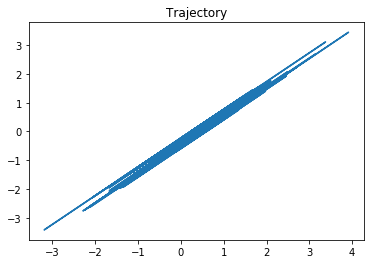
\includegraphics[width=\textwidth]{./plots/p5.png}
\caption{The trajectory of Hamiltonian HMC sampled from bivariate normal distribution with correlation 0.998.}
\label{fig_p5}
\end{figure}

\end{enumerate}

\bibliographystyle{acm}
\bibliography{reference}
\end{document}